\section{Auswertung}
\label{sec:Auswertung}

\begin{table}[H]
  \centering
  \caption{Messdaten zum Alpha-Zerfall bei einem Abstand von $x_0=1,7 cm.$}
  \label{tab:Brechungsindex}
  \sisetup{table-format=1.2}
  \begin{tabular}{S[table-format=4.0] S[table-format=6.0] S[table-format=4.0] S S}
  \toprule
  \multicolumn{1}{p{2cm}}{Luftdruck $ p / \si{\milli\bar}$} &\multicolumn{1}{p{2cm}} {Anzahl $N$ der Intensitätsmaxima} & \multicolumn{1}{p{2cm}}{Kanal des Energiemaximums} &\multicolumn{1}{p{2cm}} {effektiver Abstand $x / \si{\centi\meter}$} &\multicolumn{1}{p{2cm}} {Energie $E / \si{\mega\eV}$}\\
  \midrule
    0    & 162524 & 1023  & 0     & 4.00 \\
    50   & 163290 & 960   & 0.08  & 3.75 \\
    100  & 163917 & 1039  & 0.17  & 4.06 \\
    150  & 165093 & 1023  & 0.25  & 4.00 \\
    200  & 165693 & 1023  & 0.34  & 4.00 \\
    250  & 164583 & 1023  & 0.42  & 4.00 \\
    300  & 166084 & 1023  & 0.50  & 4.00 \\
    350  & 170833 & 1039  & 0.59  & 4.06 \\
    400  & 169738 & 1023  & 0.67  & 4.00 \\
    450  & 170667 & 1007  & 0.76  & 3.94 \\
    500  & 170908 & 1023  & 0.84  & 4.00 \\
    550  & 170471 & 1023  & 0.92  & 4.00 \\
    600  & 170319 & 1023  & 1.01  & 4.00 \\
    650  & 169636 & 975   & 1.09  & 3.81 \\
    700  & 158958 & 911   & 1.17  & 3.56 \\
    750  & 158632 & 903   & 1.26  & 3.53 \\
    800  & 156749 & 879   & 1.34  & 3.44 \\
    850  & 153795 & 847   & 1.43  & 3.31 \\
    900  & 150817 & 847   & 1.51  & 3.31 \\
    950  & 147773 & 815   & 1.59  & 3.19 \\
    1000 & 144032 & 803   & 1.68  & 3.14 \\
  \bottomrule
  \end{tabular}
\end{table}
\begin{figure}[H]
  \centering
  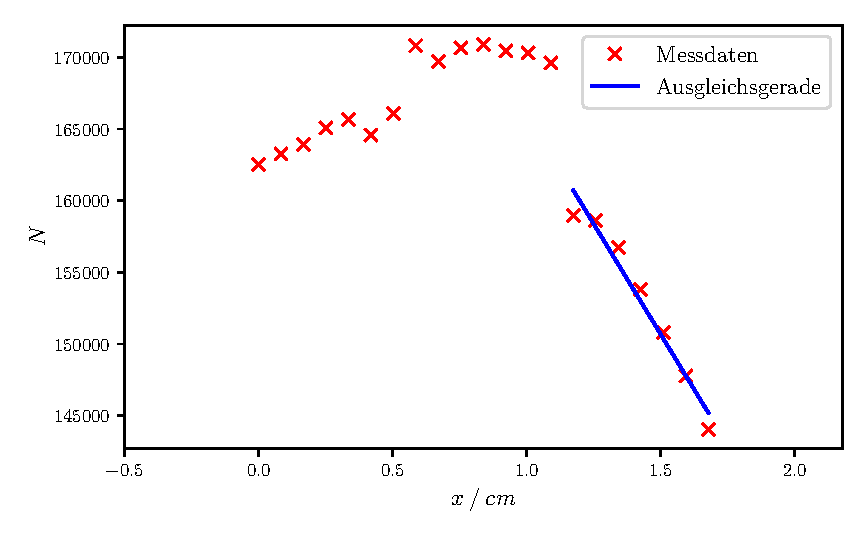
\includegraphics[width=\textwidth]{build/plot1.pdf}
  \caption {Messdaten zur Bestimmung der mittleren Reichweite aus der Zählrate (Messreihe 1).}
  \label{fig:plot1}
\end{figure}
\begin{align*}
m =& -30827.54801545226 ± 2675.7342899842047\\
b =& 196939.285880172 ± 3843.140616824728
\end{align*}


\begin{table}[H]
  \centering
  \caption{Messdaten zum Alpha-Zerfall bei einem Abstand von $x_0=3 cm.$}
  \label{tab:Brechungsindex}
  \sisetup{table-format=2.2}
  \begin{tabular}{S[table-format=4.0] S[table-format=6.0] S[table-format=4.0] S S}
    \toprule
    \multicolumn{1}{p{2cm}}{Luftdruck $ p / \si{\milli\bar}$} &\multicolumn{1}{p{2cm}} {Anzahl $N$ der Intensitätsmaxima} & \multicolumn{1}{p{2cm}}{Kanal des Energiemaximums} &\multicolumn{1}{p{2cm}} {effektiver Abstand $x / \si{\centi\meter}$} &\multicolumn{1}{p{2cm}} {Energie $E / \si{\mega\eV}$}\\
    \midrule
    0    & 55548 & 1107 & 0.00 & 4.00\\
    50   & 54994 & 1023 & 0.15 & 3.70 \\
    100  & 54486 & 1023 & 0.30 & 3.70 \\
    150  & 54186 & 987  & 0.44 & 3.57 \\
    200  & 53546 & 911  & 0.59 & 3.29 \\
    250  & 52861 & 911  & 0.74 & 3.29 \\
    300  & 52766 & 896  & 0.89 & 3.24 \\
    350  & 51527 & 896  & 1.04 & 3.24 \\
    400  & 50461 & 847  & 1.18 & 3.06 \\
    450  & 48665 & 847  & 1.33 & 3.06 \\
    500  & 45128 & 847  & 1.48 & 3.06 \\
    550  & 40047 & 751  & 1.63 & 2.71 \\
    600  & 42233 & 719  & 1.78 & 2.60 \\
    650  & 44238 & 655  & 1.92 & 2.37 \\
    700  & 33459 & 652  & 2.07 & 2.36 \\
    750  & 7126  & 688  & 2.22 & 2.49 \\
    800  & 1878  & 687  & 2.37 & 2.48 \\
    850  & 195   & 687  & 2.52 & 2.48 \\
    900  & 67    & 686  & 2.67 & 2.48 \\
    950  & 28    & 686  & 2.81 & 2.48 \\
    1000 & 23    & 686  & 2.96 & 2.48 \\
  \bottomrule
  \end{tabular}
\end{table}

\begin{figure}[H]
  \centering
  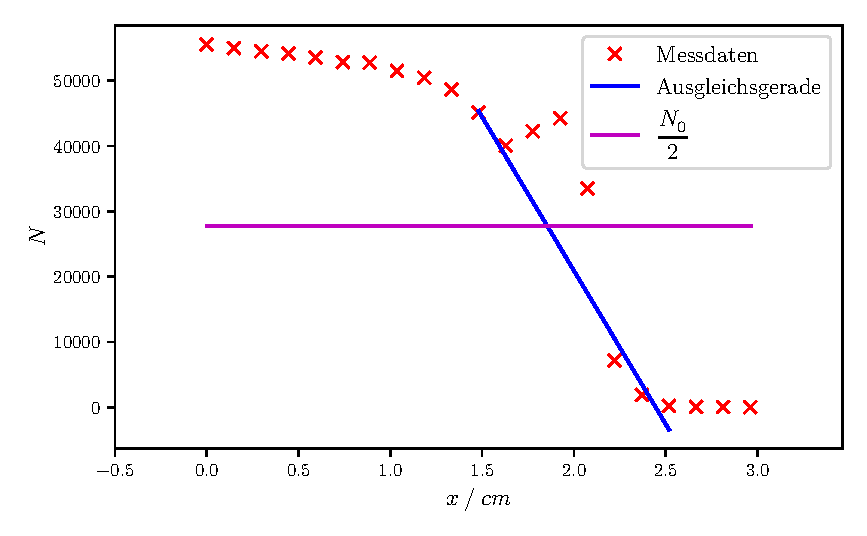
\includegraphics[width=\textwidth]{build/plot2.pdf}
  \caption {Messdaten zur Bestimmung der mittleren Reichweite aus der Zählrate (Messreihe 2).}
  \label{fig:plot2}
\end{figure}
\begin{align*}
  m_2 =& -47049.01125929326 ± 3437.2394985987107\\
  b_2 =& 115016.41234623596 ± 7165.449321747656
\end{align*}



Die Energie wird dadurch bestimmt, dass der jeweils höchste Channel dem
Energiewert $\SI{4}{\mega\eV}$ entspricht und die restlichen Channel und Energien
proportional dazu sind.

\begin{figure}[H]
  \centering
  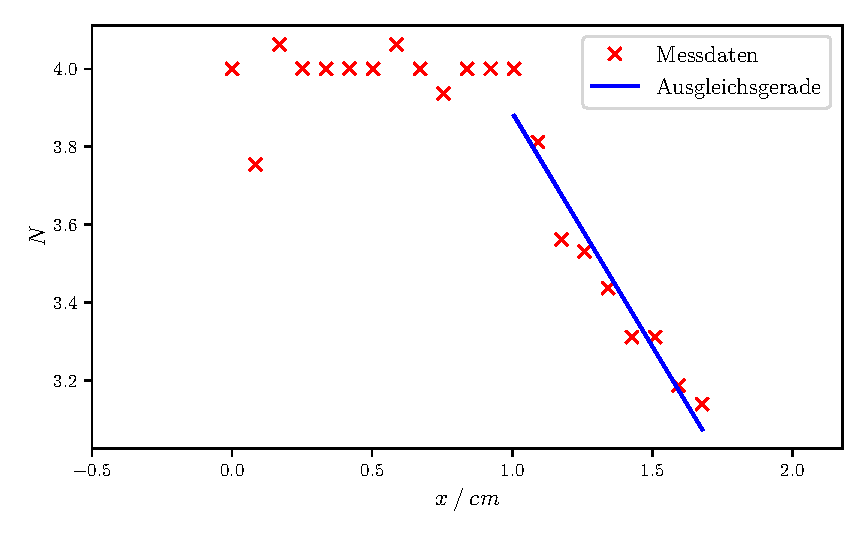
\includegraphics[width=\textwidth]{build/plot3.pdf}
  \caption {Bestimmung des Energieverlustes aus den Messdaten (Messreihe 1).}
  \label{fig:plot3}
\end{figure}

a = -1.1991428506850923 ± 0.12030234858146971
b = 5.08682524034627 ± 0.16360104210605575

\begin{figure}[H]
  \centering
  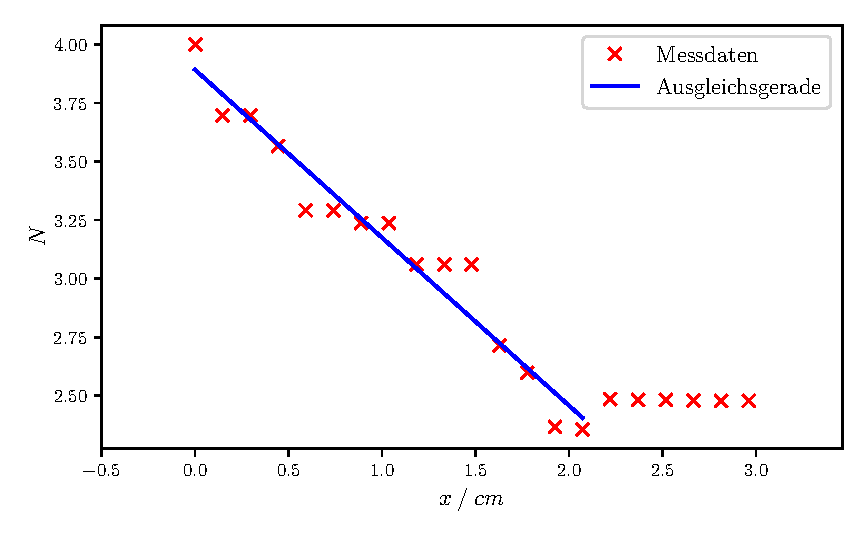
\includegraphics[width=\textwidth]{build/plot4.pdf}
  \caption {Bestimmung des Energieverlustes aus den Messdaten (Messreihe 2).}
  \label{fig:plot4}
\end{figure}


a2 = -0.7169043744199818 ± 0.04428392181469865
b2 = 3.892020475409914 ± 0.05394053882875626


\begin{figure}[H]
  \centering
  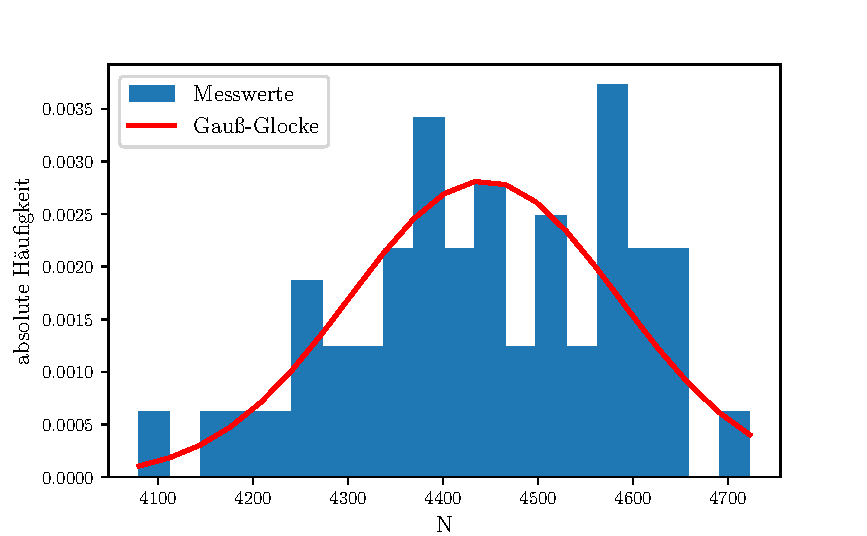
\includegraphics[width=\textwidth]{build/gauss.pdf}
  \caption {Häufigkeitsverteilung der Messwerte.}
  \label{fig:gauss}
\end{figure}
\begin{align*}
  4443.47\\
   141.7019728161891
\end{align*}

\begin{align*}
  \mu &= \frac{1}{n} \sum_{i=1}^n N_i = 4443,47\\
  \sigma &= \sqrt{ \frac{1}{n-1} \sum_{i=1}^n (N_i - \mu)^2  } =141,70
\end{align*}

\begin{align*}
  G(N, \mu, \sigma) = \frac{1}{\sigma \sqrt{2 \pi}} \cdot \text{exp} \left(- \frac{(N - \mu)^2}{2 \sigma^2} \right) \; .
\end{align*}

Um die Poissonverteilung zu berechnen werden die Werte zuerst normiert
\begin{align*}
  N_\text{i, norm} = \frac{N_i - N_\text{min}}{n}.
\end{align*}


\begin{figure}[H]
  \centering
  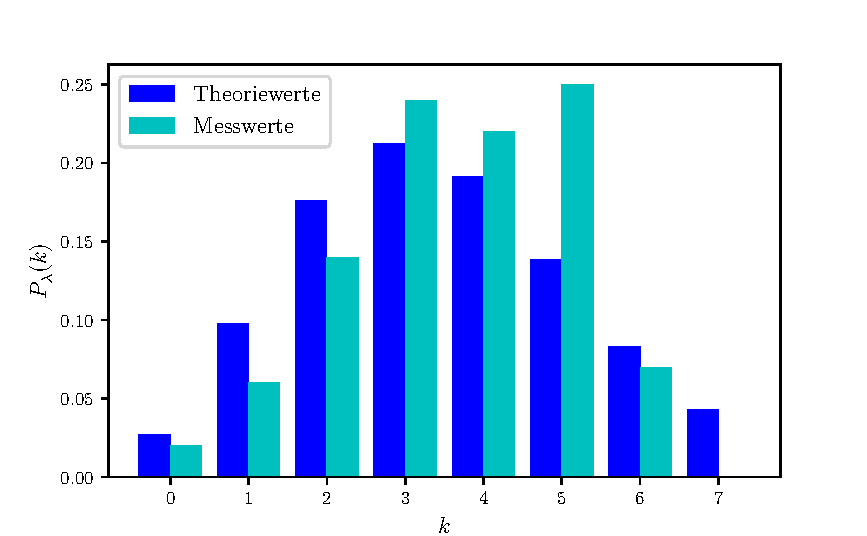
\includegraphics[width=\textwidth]{build/poisson.pdf}
  \caption {Häufigkeitsverteilung der Messwerte.}
  \label{fig:poisson}
\end{figure}

3.61 1.4275503493747603

[3. 2. 5. 2. 4. 0. 1. 2. 4. 3. 4. 2. 2. 6. 3. 6. 3. 5. 5. 4. 4. 4. 3. 4.
 5. 5. 2. 4. 5. 3. 5. 2. 4. 5. 3. 3. 1. 4. 3. 5. 3. 3. 2. 5. 1. 5. 5. 2.
 4. 3. 4. 6. 4. 5. 4. 3. 6. 4. 2. 5. 3. 1. 0. 5. 2. 3. 3. 5. 5. 6. 5. 5.
 3. 4. 1. 5. 4. 5. 4. 5. 3. 4. 4. 4. 4. 2. 3. 2. 3. 3. 5. 3. 5. 5. 6. 2.
 3. 1. 3. 6.]